\documentclass{standalone}
\usepackage{tikz}
\usetikzlibrary{patterns, positioning}

\begin{document}
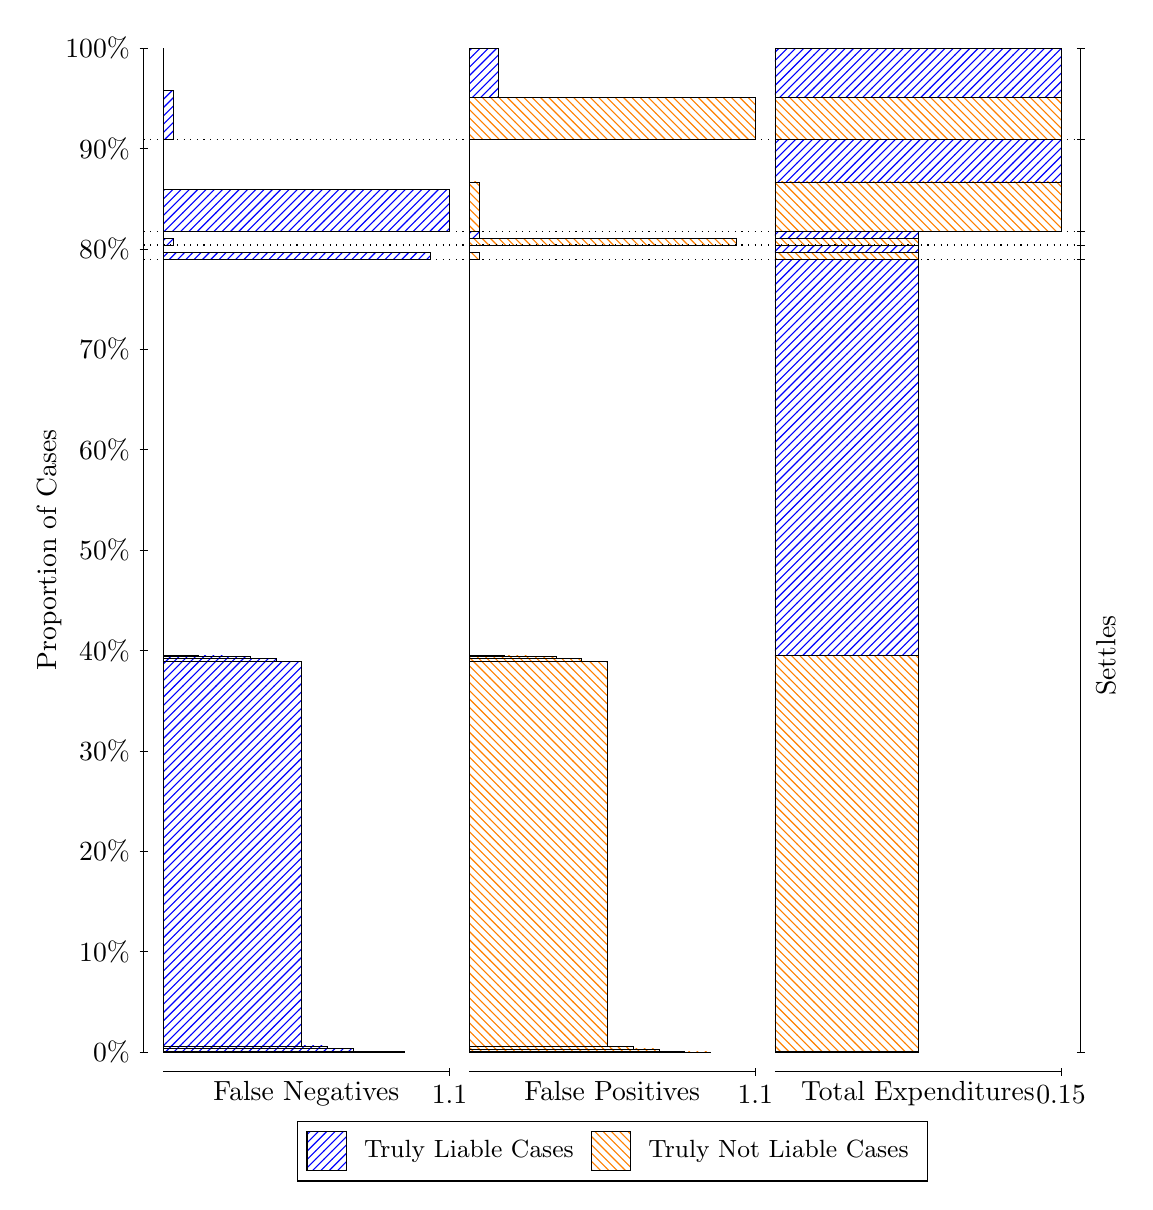
\begin{tikzpicture}
\draw[black, very thin] (1.5,1.75) -- (1.5,14.5);
\node[rotate=90, anchor=center] at (0.3, 8.125) {Proportion of Cases};
\draw[black, very thin] (1.45,1.75) -- (1.55,1.75);
\node[anchor=east] at (1.45, 1.75) {0\%};
\draw[black, very thin] (1.45,3.025) -- (1.55,3.025);
\node[anchor=east] at (1.45, 3.025) {10\%};
\draw[black, very thin] (1.45,4.3) -- (1.55,4.3);
\node[anchor=east] at (1.45, 4.3) {20\%};
\draw[black, very thin] (1.45,5.575) -- (1.55,5.575);
\node[anchor=east] at (1.45, 5.575) {30\%};
\draw[black, very thin] (1.45,6.85) -- (1.55,6.85);
\node[anchor=east] at (1.45, 6.85) {40\%};
\draw[black, very thin] (1.45,8.125) -- (1.55,8.125);
\node[anchor=east] at (1.45, 8.125) {50\%};
\draw[black, very thin] (1.45,9.4) -- (1.55,9.4);
\node[anchor=east] at (1.45, 9.4) {60\%};
\draw[black, very thin] (1.45,10.675) -- (1.55,10.675);
\node[anchor=east] at (1.45, 10.675) {70\%};
\draw[black, very thin] (1.45,11.95) -- (1.55,11.95);
\node[anchor=east] at (1.45, 11.95) {80\%};
\draw[black, very thin] (1.45,13.225) -- (1.55,13.225);
\node[anchor=east] at (1.45, 13.225) {90\%};
\draw[black, very thin] (1.45,14.5) -- (1.55,14.5);
\node[anchor=east] at (1.45, 14.5) {100\%};

\draw[black, very thin] (13.4,1.75) -- (13.4,14.5);
\draw[black, very thin] (13.35,1.75) -- (13.45,1.75);
\node[anchor=west] at (13.35, 1.75) {};
\draw[black, very thin] (13.35,11.815) -- (13.45,11.815);
\node[anchor=west] at (13.35, 11.815) {};
\draw[black, very thin] (13.35,11.998) -- (13.45,11.998);
\node[anchor=west] at (13.35, 11.998) {};
\draw[black, very thin] (13.35,12.17) -- (13.45,12.17);
\node[anchor=west] at (13.35, 12.17) {};
\draw[black, very thin] (13.35,13.335) -- (13.45,13.335);
\node[anchor=west] at (13.35, 13.335) {};
\draw[black, very thin] (13.35,14.5) -- (13.45,14.5);
\node[anchor=west] at (13.35, 14.5) {};

\draw[black, very thin, pattern color=blue, pattern=north east lines] (1.75,1.75) rectangle (4.8118,1.754);
\draw[black, very thin, pattern color=blue, pattern=north east lines] (1.75,1.754) rectangle (4.4852,1.7548);
\draw[black, very thin, pattern color=blue, pattern=north east lines] (1.75,1.7548) rectangle (4.1586,1.791);
\draw[black, very thin, pattern color=blue, pattern=north east lines] (1.75,1.791) rectangle (3.832,1.8267);
\draw[black, very thin, pattern color=blue, pattern=north east lines] (1.75,1.8267) rectangle (3.5054,6.7117);
\draw[black, very thin, pattern color=blue, pattern=north east lines] (1.75,6.7117) rectangle (3.1788,6.744);
\draw[black, very thin, pattern color=blue, pattern=north east lines] (1.75,6.744) rectangle (2.8522,6.778);
\draw[black, very thin, pattern color=blue, pattern=north east lines] (1.75,6.778) rectangle (2.5257,6.7797);
\draw[black, very thin, pattern color=blue, pattern=north east lines] (1.75,6.7797) rectangle (2.1991,6.782);
\draw[black, very thin, pattern color=orange, pattern=north west lines] (1.75,6.782) rectangle (1.75,11.815);
\draw[black, very thin, pattern color=blue, pattern=north east lines] (1.75,11.815) rectangle (5.1384,11.909);
\draw[black, very thin, pattern color=orange, pattern=north west lines] (1.75,11.909) rectangle (1.75,11.998);
\draw[black, very thin, pattern color=blue, pattern=north east lines] (1.75,11.998) rectangle (1.8725,12.082);
\draw[black, very thin, pattern color=orange, pattern=north west lines] (1.75,12.082) rectangle (1.75,12.17);
\draw[black, very thin, pattern color=blue, pattern=north east lines] (1.75,12.17) rectangle (5.3833,12.705);
\draw[black, very thin, pattern color=orange, pattern=north west lines] (1.75,12.705) rectangle (1.75,13.335);
\draw[black, very thin, pattern color=blue, pattern=north east lines] (1.75,13.335) rectangle (1.8725,13.965);
\draw[black, very thin, pattern color=orange, pattern=north west lines] (1.75,13.965) rectangle (1.75,14.5);
\draw[black, very thin, pattern color=orange, pattern=north west lines] (5.6333,1.75) rectangle (8.6951,1.7523);
\draw[black, very thin, pattern color=orange, pattern=north west lines] (5.6333,1.7523) rectangle (8.3685,1.7541);
\draw[black, very thin, pattern color=orange, pattern=north west lines] (5.6333,1.7541) rectangle (8.0419,1.7896);
\draw[black, very thin, pattern color=orange, pattern=north west lines] (5.6333,1.7896) rectangle (7.7154,1.8234);
\draw[black, very thin, pattern color=orange, pattern=north west lines] (5.6333,1.8234) rectangle (7.3888,6.7102);
\draw[black, very thin, pattern color=orange, pattern=north west lines] (5.6333,6.7102) rectangle (7.0622,6.744);
\draw[black, very thin, pattern color=orange, pattern=north west lines] (5.6333,6.744) rectangle (7.0622,6.7443);
\draw[black, very thin, pattern color=orange, pattern=north west lines] (5.6333,6.7443) rectangle (6.7356,6.7787);
\draw[black, very thin, pattern color=orange, pattern=north west lines] (5.6333,6.7787) rectangle (6.409,6.7795);
\draw[black, very thin, pattern color=orange, pattern=north west lines] (5.6333,6.7795) rectangle (6.0824,6.7833);
\draw[black, very thin, pattern color=blue, pattern=north east lines] (5.6333,6.7833) rectangle (5.6333,11.815);
\draw[black, very thin, pattern color=orange, pattern=north west lines] (5.6333,11.815) rectangle (5.7558,11.904);
\draw[black, very thin, pattern color=blue, pattern=north east lines] (5.6333,11.904) rectangle (5.6333,11.998);
\draw[black, very thin, pattern color=orange, pattern=north west lines] (5.6333,11.998) rectangle (9.0217,12.086);
\draw[black, very thin, pattern color=blue, pattern=north east lines] (5.6333,12.086) rectangle (5.7558,12.17);
\draw[black, very thin, pattern color=orange, pattern=north west lines] (5.6333,12.17) rectangle (5.7558,12.8);
\draw[black, very thin, pattern color=blue, pattern=north east lines] (5.6333,12.8) rectangle (5.6333,13.335);
\draw[black, very thin, pattern color=orange, pattern=north west lines] (5.6333,13.335) rectangle (9.2667,13.87);
\draw[black, very thin, pattern color=blue, pattern=north east lines] (5.6333,13.87) rectangle (6.0007,14.5);
\draw[black, very thin, pattern color=orange, pattern=north west lines] (9.5167,1.75) rectangle (11.333,1.7545);
\draw[black, very thin, pattern color=blue, pattern=north east lines] (9.5167,1.7545) rectangle (11.333,1.7593);
\draw[black, very thin, pattern color=orange, pattern=north west lines] (9.5167,1.7593) rectangle (11.333,6.788);
\draw[black, very thin, pattern color=blue, pattern=north east lines] (9.5167,6.788) rectangle (11.333,11.815);
\draw[black, very thin, pattern color=orange, pattern=north west lines] (9.5167,11.815) rectangle (11.333,11.904);
\draw[black, very thin, pattern color=blue, pattern=north east lines] (9.5167,11.904) rectangle (11.333,11.998);
\draw[black, very thin, pattern color=orange, pattern=north west lines] (9.5167,11.998) rectangle (11.333,12.086);
\draw[black, very thin, pattern color=blue, pattern=north east lines] (9.5167,12.086) rectangle (11.333,12.17);
\draw[black, very thin, pattern color=orange, pattern=north west lines] (9.5167,12.17) rectangle (13.15,12.8);
\draw[black, very thin, pattern color=blue, pattern=north east lines] (9.5167,12.8) rectangle (13.15,13.335);
\draw[black, very thin, pattern color=orange, pattern=north west lines] (9.5167,13.335) rectangle (13.15,13.87);
\draw[black, very thin, pattern color=blue, pattern=north east lines] (9.5167,13.87) rectangle (13.15,14.5);
\draw[black, dotted] (1.5,11.815) -- (13.4,11.815);
\draw[black, dotted] (1.5,11.998) -- (13.4,11.998);
\draw[black, dotted] (1.5,12.17) -- (13.4,12.17);
\draw[black, dotted] (1.5,13.335) -- (13.4,13.335);
\draw[black, very thin] (1.75,1.5) -- (5.3833,1.5);
\node[anchor=north] at (3.5667, 1.5) {False Negatives};
\draw[black, very thin] (5.3833,1.45) -- (5.3833,1.55);
\node[anchor=north] at (5.3833, 1.45) {1.1};

\draw[black, very thin] (5.6333,1.5) -- (9.2667,1.5);
\node[anchor=north] at (7.45, 1.5) {False Positives};
\draw[black, very thin] (9.2667,1.45) -- (9.2667,1.55);
\node[anchor=north] at (9.2667, 1.45) {1.1};

\draw[black, very thin] (9.5167,1.5) -- (13.15,1.5);
\node[anchor=north] at (11.333, 1.5) {Total Expenditures};
\draw[black, very thin] (13.15,1.45) -- (13.15,1.55);
\node[anchor=north] at (13.15, 1.45) {0.15};

\node[black, centered, rotate=90] at (13.72, 6.7826) {Settles};





\draw (7.449999999999999,1.5) node[draw=none] (baseCoordinate) {};
\begin{scope}[align=center]
        \matrix[scale=0.5, draw=black, below=0.5cm of baseCoordinate, nodes={draw}, column sep=0.1cm]{
            \node[rectangle, draw, minimum width=0.5cm, minimum height=0.5cm, pattern=north east lines, pattern color=blue] {}; &
            \node[draw=none, font=\small] (B) {Truly Liable Cases}; &
            \node[rectangle, draw, minimum width=0.5cm, minimum height=0.5cm, pattern=north west lines, pattern color=orange] {}; &
            \node[draw=none, font=\small] (B) {Truly Not Liable Cases}; \\
            };
\end{scope}

\end{tikzpicture}
\end{document}